\subsection{Vorlesungskalender mit Google Calendar}\label{ch:GC}
Damit der Studiengangsleiter die Vorlesungen organisieren kann, wird der Google Calendar gemäß der Anforderung A2 und A3 aus der Tabelle \vref{anf:GC} vollständig in die Software integriert.
Damit die Ereignisse der jeweiligen Google Calendar angezeigt sowie verwaltet werden können, muss ein Kalender in React implementiert werden. 

\subsubsection{Einbindung des DevExtreme React Scheduler}
Der \textit{DevExtreme React Scheduler}\footnote{\url{https://devexpress.github.io/devextreme-reactive/react/scheduler/}} ist eine Komponente für Material-UI, die einen Kalender für React bereitstellt. 
Das Erscheinungsbild des React Schedulers ist von dem Google Calendar inspiriert und benutzerfreundlich gestaltet.\autocite[Vgl.][]{ReactScheduler} 
Neben Funktionalitäten, wie beispielsweise Drag-and-Drop-Operationen sowie unterschiedlichen Anzeigeoptionen, ist insbesondere die Anbindung und Integration eines Google Calendars über geeignete Schnittstellen ausschlaggebend für die Entscheidung zur Verwendung der Komponente. 

In Abbildung \vref{fig:ReactScheduler} ist eine Übersicht mit erklärenden Ergänzungen über den implementierten und konfigurierten React Scheduler dargestellt. 
Zur Verwendung des React Schedulers wird ein Package und entsprechende Abhängigkeiten von NPM eingebunden.\footnote{\url{https://www.npmjs.com/package/@devexpress/dx-react-scheduler}}
Weitere Informationen zur Einbindung sowie Konfiguration des Kalenders sind in der Dokumentation von DevExtreme gegeben.\footnote{\url{https://devexpress.github.io/devextreme-reactive/react/scheduler/docs/guides/getting-started/}}
\begin{figure}[H]
	\centering 
	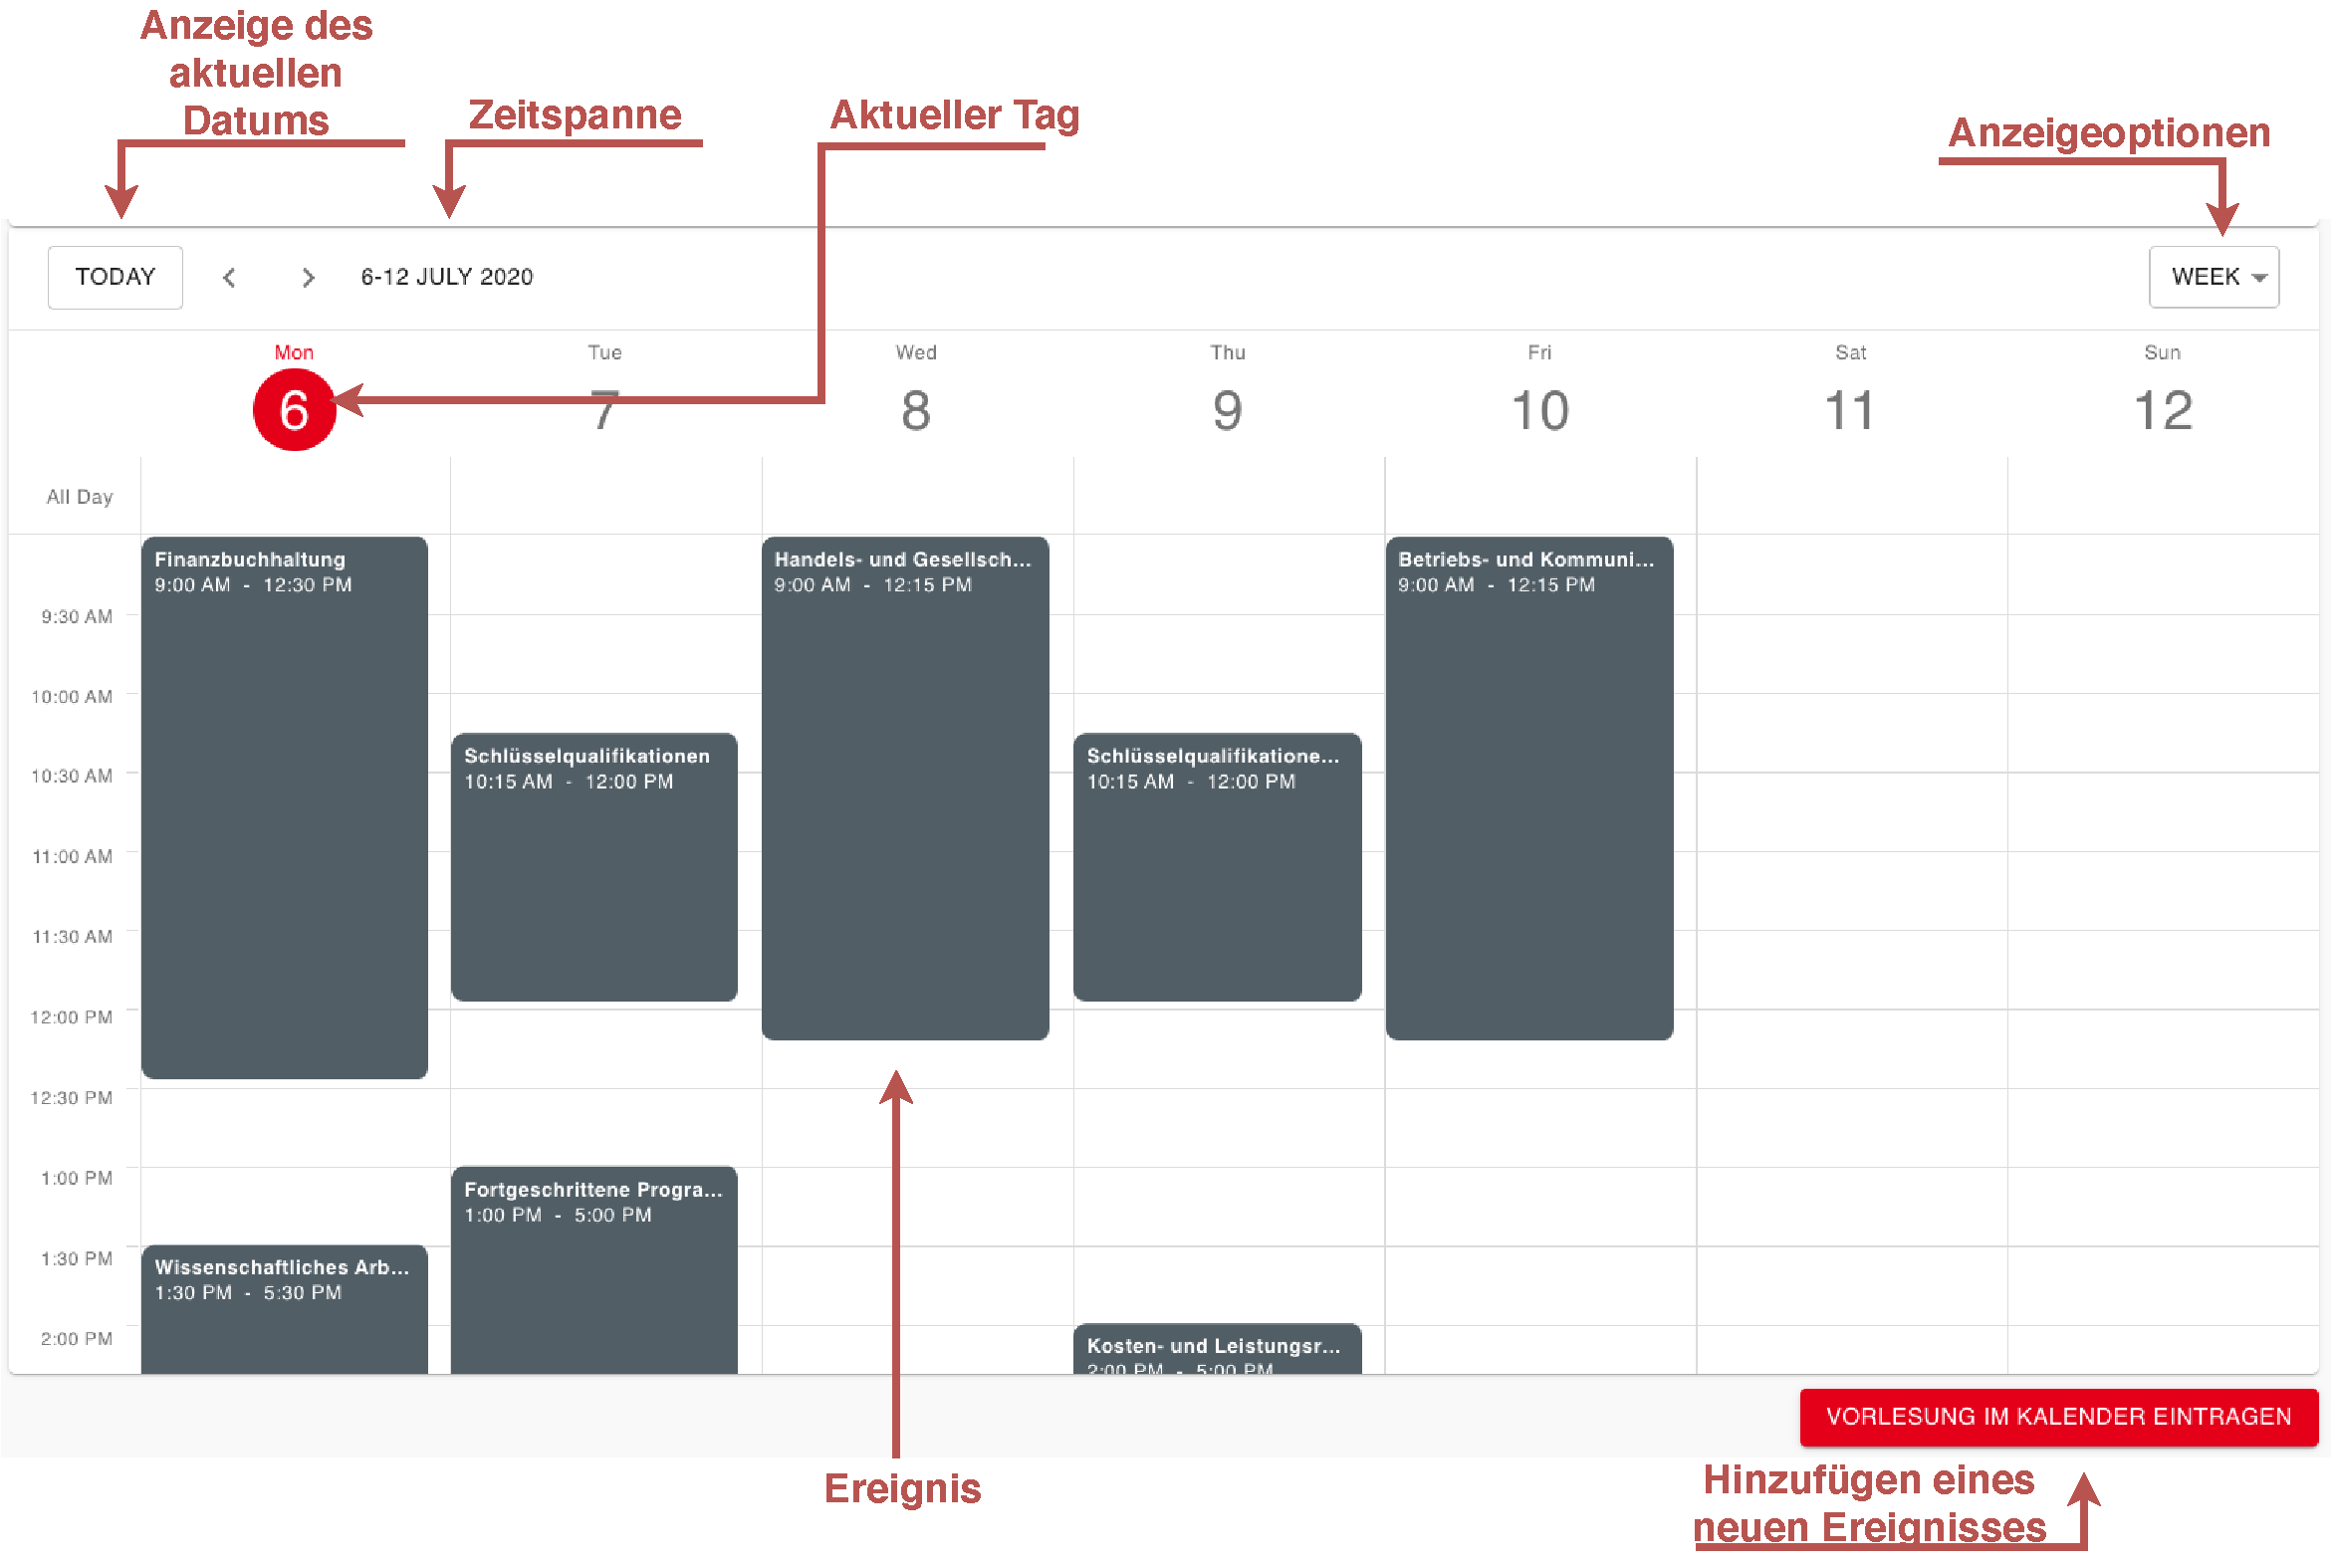
\includegraphics[width=\textwidth]{img/FrontEnd/ReactCalendar.pdf}
	\caption[Übersicht des React Schedulers]{\label{fig:ReactScheduler}Übersicht des React Schedulers}
\end{figure}

\subsubsection{Initialisierung und Verbindung des Google Calendars}
Der Google Calendar ermöglicht eine Anbindung an das System über eine \ac{API}.
Damit die Inhalte eines Google Calendars über die Google Calendar-\ac{API}-Schnittstelle\footnote{\url{https://developers.google.com/calendar/v3/reference}} angefragt und in dem React Scheduler angezeigt werden können, müssen die Anfragen über einen Token authentifiziert werden. 
Hierfür wird OAuth 2.0 verwendet, um die Authentifizierung durchzuführen.\autocite[Vgl.][]{GCApi} 

In einer eigenen JavaScript-Datei \texttt{apiHandlerGoogleCalendar.js} wird der Token bei den Anfragen mitgegeben. Dieser Token wird nach einem einmaligen Bestätigen des Zugriffs auf den Google Calendar erstellt und hinterlegt. 
Mit einem validen Token werden die Anfragen an die Google Calendar-\ac{API} genehmigt und die Inhalte des jeweiligen Kalenders an die Anwendung übertragen. Die erhaltenen Inhalte werden formatiert und in dem React Scheduler angezeigt.


\subsubsection{Interaktion mit dem Kalender}\label{ch:InteraktionGC}
Zur Funktionalität des Kalenders werden drei unterschiedliche Interaktionen mit dem Google Calendar benötigt: das Hinzufügen, das Ändern sowie das Löschen von Ereignissen. Im Folgenden werden die Anfragen an die \ac{REST}-\ac{API} des Google Calendars näher beschrieben.

\textbf{Hinzufügen von Ereignissen}\newline
In dem React Scheduler können neue Ereignisse dem Kalender hinzugefügt werden.
In Abbildung \vref{fig:AddReactScheduler} ist das Dialog-Fenster abgebildet, welches nach dem Drücken des Hinzufügebuttons erscheint.
\begin{figure}[H]
	\centering 
	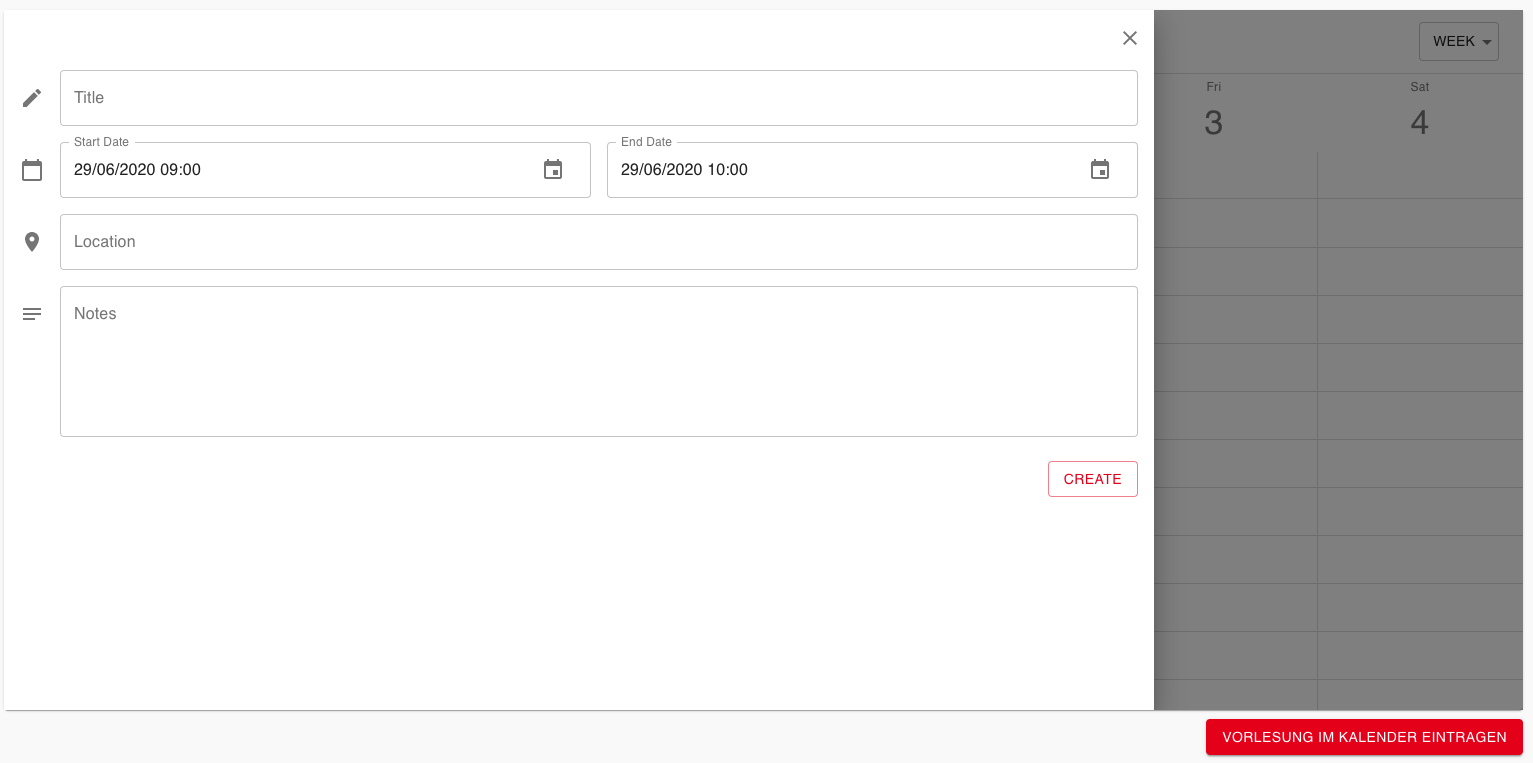
\includegraphics[width=\textwidth]{img/FrontEnd/GCAdd.png}
	\caption[Erstellen eines Ereignisses im React Scheduler]{\label{fig:AddReactScheduler}Erstellen eines Ereignisses im React Scheduler}
\end{figure}

Zusätzlich zu den abgebildeten Inhalten werden die Kalender-ID und der Token bei der PUSH-Anfrage übermittelt. Hierbei wird die Bibliothek \textit{GAPI} von Google verwendet, die eine einfache Verbindung mit der \ac{API} über browserseitiges JavaScript ermöglicht. 
Eine detaillierte Dokumentation dieser Anfrage ist in der Schnittstellenbeschreibung der Google Calendar \ac{API} gegeben.\footnote{\url{https://developers.google.com/calendar/v3/reference/events/insert}}

\textbf{Ändern von Ereignisssen}\newline
Vorhandene Ereignisse können ebenfalls bearbeitet werden, indem die entsprechende Veranstaltung ausgewält und der Bearbeiten-Button auf dem erscheinenden Popup geklickt wird, welches in Abbildung \vref{fig:GCPopup} dargestellt ist. 
\begin{figure}[H]
	\centering 
	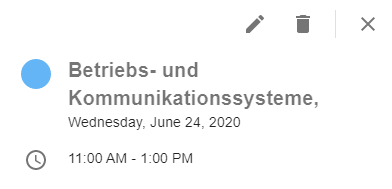
\includegraphics[width=6cm]{img/FrontEnd/GCPopup.png}
	\caption[Popup eines Ereignisses im React Scheduler]{\label{fig:GCPopup}Popup eines Ereignisses im React Scheduler}
\end{figure}

Zur Änderung der Daten wird eine \ac{API}-Anfrage mit der Methode \textit{update} verwendet.\footnote{\url{https://developers.google.com/calendar/v3/reference/events/update}} 
Diese ist vom Aufbau ähnlich zu der zuvor vorgestellten \textit{insert}-Methode.

\textbf{Löschen von Ereignissen}\newline
Zusätzlich können Ereignisse in dem Google Calendar gelöscht werden, indem die Funktionalität, ebenfalls in Abbildung \vref{fig:GCPopup} abgebildet, genutzt wird. 
Zur Durchführung dieser Operation wird das Event \textit{delete} verwendet, wobei lediglich die Calendar-ID sowie die Event-ID übermittelt werden.\footnote{\url{https://developers.google.com/calendar/v3/reference/events/delete}}   
In dem Code-Ausschnitt \vref{lst:deleteEvent} ist die Erstellung der Delete-Anfrage abgebildet.

%TODO Formatting and Coloring JavaScript-Code
\lstset{language=JavaScript}
\begin{lstlisting}[caption={Anfrage zum Löschen eines Ereignisses}, label={lst:deleteEvent}]
function handleAppointmentDelete(deleteAppointmentId, gapi) {
  var request = gapi.client.calendar.events.delete({
    'calendarId': creds.calenderID,
    'eventId': deleteAppointmentId
  });

  request.execute(function (response) {
    if (response.error || response == false) {
      alert('Error');
    } else {
      alert('Success');
    }
  });
}
\end{lstlisting}

%TODO \subsubsection{Ausblick GC}
%Mit dieser Integration der Inhalte des Google Calendars, können die Inhalte dargestellt und verändert werden. 
%Durch die Schnittstellen-Kommuniktaion ist jedoch ein paralleles Bearbeiten des Google Calendars, in der vorliegenden Anwendung sowie in dem Google Calendar direkt, möglich. 
%Dieses Szenario ist jedoch als sehr selten
